\documentclass{standalone}
\usepackage{tikz}
\usetikzlibrary{patterns, positioning}

\begin{document}
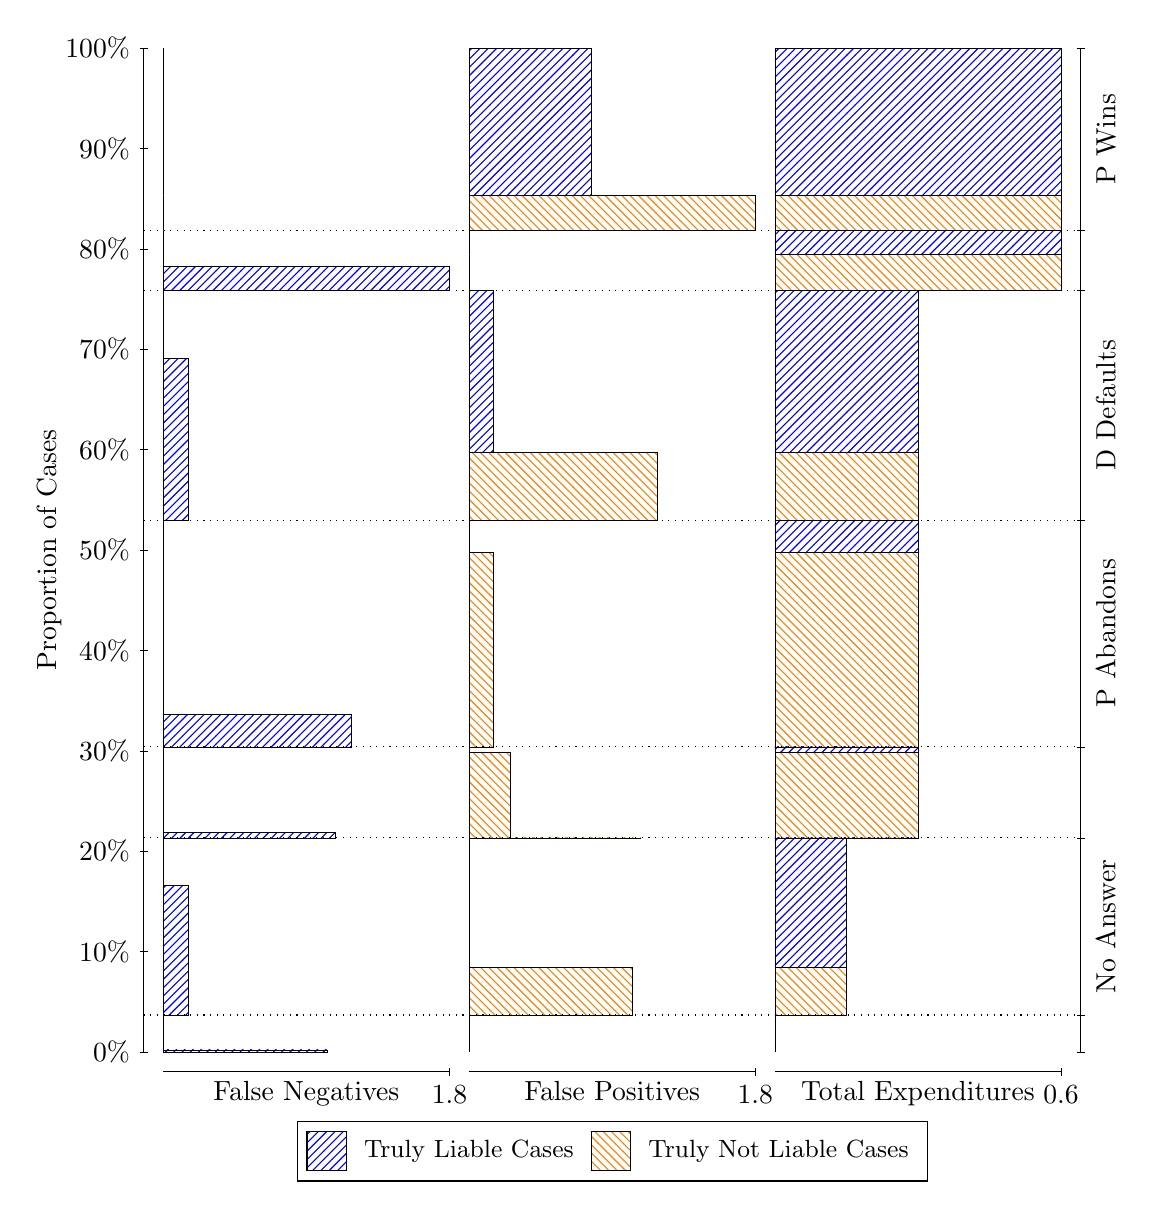
\begin{tikzpicture}
\draw[black, very thin] (1.5,1.75) -- (1.5,14.5);
\node[rotate=90, anchor=center] at (0.3, 8.125) {Proportion of Cases};
\draw[black, very thin] (1.45,1.75) -- (1.55,1.75);
\node[anchor=east] at (1.45, 1.75) {0\%};
\draw[black, very thin] (1.45,3.025) -- (1.55,3.025);
\node[anchor=east] at (1.45, 3.025) {10\%};
\draw[black, very thin] (1.45,4.3) -- (1.55,4.3);
\node[anchor=east] at (1.45, 4.3) {20\%};
\draw[black, very thin] (1.45,5.575) -- (1.55,5.575);
\node[anchor=east] at (1.45, 5.575) {30\%};
\draw[black, very thin] (1.45,6.85) -- (1.55,6.85);
\node[anchor=east] at (1.45, 6.85) {40\%};
\draw[black, very thin] (1.45,8.125) -- (1.55,8.125);
\node[anchor=east] at (1.45, 8.125) {50\%};
\draw[black, very thin] (1.45,9.4) -- (1.55,9.4);
\node[anchor=east] at (1.45, 9.4) {60\%};
\draw[black, very thin] (1.45,10.675) -- (1.55,10.675);
\node[anchor=east] at (1.45, 10.675) {70\%};
\draw[black, very thin] (1.45,11.95) -- (1.55,11.95);
\node[anchor=east] at (1.45, 11.95) {80\%};
\draw[black, very thin] (1.45,13.225) -- (1.55,13.225);
\node[anchor=east] at (1.45, 13.225) {90\%};
\draw[black, very thin] (1.45,14.5) -- (1.55,14.5);
\node[anchor=east] at (1.45, 14.5) {100\%};

\draw[black, very thin] (13.4,1.75) -- (13.4,14.5);
\draw[black, very thin] (13.35,1.75) -- (13.45,1.75);
\node[anchor=west] at (13.35, 1.75) {};
\draw[black, very thin] (13.35,2.2192) -- (13.45,2.2192);
\node[anchor=west] at (13.35, 2.2192) {};
\draw[black, very thin] (13.35,4.4702) -- (13.45,4.4702);
\node[anchor=west] at (13.35, 4.4702) {};
\draw[black, very thin] (13.35,5.6259) -- (13.45,5.6259);
\node[anchor=west] at (13.35, 5.6259) {};
\draw[black, very thin] (13.35,8.5037) -- (13.45,8.5037);
\node[anchor=west] at (13.35, 8.5037) {};
\draw[black, very thin] (13.35,11.422) -- (13.45,11.422);
\node[anchor=west] at (13.35, 11.422) {};
\draw[black, very thin] (13.35,12.183) -- (13.45,12.183);
\node[anchor=west] at (13.35, 12.183) {};
\draw[black, very thin] (13.35,14.5) -- (13.45,14.5);
\node[anchor=west] at (13.35, 14.5) {};

\draw[black, very thin, pattern color=blue, pattern=north east lines] (1.75,1.75) rectangle (3.8262,1.7775);
\draw[black, very thin, pattern color=orange, pattern=north west lines] (1.75,1.7775) rectangle (1.75,2.2192);
\draw[black, very thin, pattern color=blue, pattern=north east lines] (1.75,2.2192) rectangle (2.0614,3.8644);
\draw[black, very thin, pattern color=orange, pattern=north west lines] (1.75,3.8644) rectangle (1.75,4.4702);
\draw[black, very thin, pattern color=blue, pattern=north east lines] (1.75,4.4702) rectangle (3.93,4.537);
\draw[black, very thin, pattern color=blue, pattern=north east lines] (1.75,4.537) rectangle (3.7224,4.537);
\draw[black, very thin, pattern color=blue, pattern=north east lines] (1.75,4.537) rectangle (3.5148,4.537);
\draw[black, very thin, pattern color=blue, pattern=north east lines] (1.75,4.537) rectangle (3.3071,4.537);
\draw[black, very thin, pattern color=blue, pattern=north east lines] (1.75,4.537) rectangle (3.0995,4.537);
\draw[black, very thin, pattern color=blue, pattern=north east lines] (1.75,4.537) rectangle (2.8919,4.537);
\draw[black, very thin, pattern color=blue, pattern=north east lines] (1.75,4.537) rectangle (2.6843,4.537);
\draw[black, very thin, pattern color=blue, pattern=north east lines] (1.75,4.537) rectangle (2.4767,4.537);
\draw[black, very thin, pattern color=blue, pattern=north east lines] (1.75,4.537) rectangle (2.269,4.537);
\draw[black, very thin, pattern color=orange, pattern=north west lines] (1.75,4.537) rectangle (1.75,5.6259);
\draw[black, very thin, pattern color=blue, pattern=north east lines] (1.75,5.6259) rectangle (4.1376,6.0331);
\draw[black, very thin, pattern color=orange, pattern=north west lines] (1.75,6.0331) rectangle (1.75,8.5037);
\draw[black, very thin, pattern color=blue, pattern=north east lines] (1.75,8.5037) rectangle (2.0614,10.557);
\draw[black, very thin, pattern color=orange, pattern=north west lines] (1.75,10.557) rectangle (1.75,11.422);
\draw[black, very thin, pattern color=blue, pattern=north east lines] (1.75,11.422) rectangle (5.3833,11.725);
\draw[black, very thin, pattern color=orange, pattern=north west lines] (1.75,11.725) rectangle (1.75,12.183);
\draw[black, very thin, pattern color=orange, pattern=north west lines] (1.75,12.183) rectangle (1.75,12.629);
\draw[black, very thin, pattern color=blue, pattern=north east lines] (1.75,12.629) rectangle (1.75,14.5);
\draw[black, very thin, pattern color=orange, pattern=north west lines] (5.6333,1.75) rectangle (5.6333,2.1917);
\draw[black, very thin, pattern color=blue, pattern=north east lines] (5.6333,2.1917) rectangle (5.6333,2.2192);
\draw[black, very thin, pattern color=orange, pattern=north west lines] (5.6333,2.2192) rectangle (7.7095,2.8249);
\draw[black, very thin, pattern color=blue, pattern=north east lines] (5.6333,2.8249) rectangle (5.6333,4.4702);
\draw[black, very thin, pattern color=orange, pattern=north west lines] (5.6333,4.4702) rectangle (7.8133,4.4702);
\draw[black, very thin, pattern color=orange, pattern=north west lines] (5.6333,4.4702) rectangle (7.6057,4.4702);
\draw[black, very thin, pattern color=orange, pattern=north west lines] (5.6333,4.4702) rectangle (7.3981,4.4702);
\draw[black, very thin, pattern color=orange, pattern=north west lines] (5.6333,4.4702) rectangle (7.1905,4.4702);
\draw[black, very thin, pattern color=orange, pattern=north west lines] (5.6333,4.4702) rectangle (6.9829,4.4702);
\draw[black, very thin, pattern color=orange, pattern=north west lines] (5.6333,4.4702) rectangle (6.7752,4.4702);
\draw[black, very thin, pattern color=orange, pattern=north west lines] (5.6333,4.4702) rectangle (6.7752,4.4702);
\draw[black, very thin, pattern color=orange, pattern=north west lines] (5.6333,4.4702) rectangle (6.5676,4.4702);
\draw[black, very thin, pattern color=orange, pattern=north west lines] (5.6333,4.4702) rectangle (6.36,4.4702);
\draw[black, very thin, pattern color=orange, pattern=north west lines] (5.6333,4.4702) rectangle (6.1524,5.5591);
\draw[black, very thin, pattern color=blue, pattern=north east lines] (5.6333,5.5591) rectangle (5.7371,5.5591);
\draw[black, very thin, pattern color=blue, pattern=north east lines] (5.6333,5.5591) rectangle (5.6333,5.6259);
\draw[black, very thin, pattern color=orange, pattern=north west lines] (5.6333,5.6259) rectangle (5.9448,8.0965);
\draw[black, very thin, pattern color=blue, pattern=north east lines] (5.6333,8.0965) rectangle (5.6333,8.5037);
\draw[black, very thin, pattern color=orange, pattern=north west lines] (5.6333,8.5037) rectangle (8.021,9.3677);
\draw[black, very thin, pattern color=blue, pattern=north east lines] (5.6333,9.3677) rectangle (5.9448,11.422);
\draw[black, very thin, pattern color=orange, pattern=north west lines] (5.6333,11.422) rectangle (5.6333,11.879);
\draw[black, very thin, pattern color=blue, pattern=north east lines] (5.6333,11.879) rectangle (5.6333,12.183);
\draw[black, very thin, pattern color=orange, pattern=north west lines] (5.6333,12.183) rectangle (9.2667,12.629);
\draw[black, very thin, pattern color=blue, pattern=north east lines] (5.6333,12.629) rectangle (7.1905,14.5);
\draw[black, very thin, pattern color=orange, pattern=north west lines] (9.5167,1.75) rectangle (9.5167,2.1917);
\draw[black, very thin, pattern color=blue, pattern=north east lines] (9.5167,2.1917) rectangle (9.5167,2.2192);
\draw[black, very thin, pattern color=orange, pattern=north west lines] (9.5167,2.2192) rectangle (10.425,2.8249);
\draw[black, very thin, pattern color=blue, pattern=north east lines] (9.5167,2.8249) rectangle (10.425,4.4702);
\draw[black, very thin, pattern color=orange, pattern=north west lines] (9.5167,4.4702) rectangle (11.333,4.4702);
\draw[black, very thin, pattern color=blue, pattern=north east lines] (9.5167,4.4702) rectangle (11.333,4.4702);
\draw[black, very thin, pattern color=orange, pattern=north west lines] (9.5167,4.4702) rectangle (11.333,5.5591);
\draw[black, very thin, pattern color=blue, pattern=north east lines] (9.5167,5.5591) rectangle (11.333,5.6259);
\draw[black, very thin, pattern color=orange, pattern=north west lines] (9.5167,5.6259) rectangle (11.333,5.6259);
\draw[black, very thin, pattern color=blue, pattern=north east lines] (9.5167,5.6259) rectangle (11.333,5.6259);
\draw[black, very thin, pattern color=orange, pattern=north west lines] (9.5167,5.6259) rectangle (11.333,8.0965);
\draw[black, very thin, pattern color=blue, pattern=north east lines] (9.5167,8.0965) rectangle (11.333,8.5037);
\draw[black, very thin, pattern color=orange, pattern=north west lines] (9.5167,8.5037) rectangle (11.333,9.3677);
\draw[black, very thin, pattern color=blue, pattern=north east lines] (9.5167,9.3677) rectangle (11.333,11.422);
\draw[black, very thin, pattern color=orange, pattern=north west lines] (9.5167,11.422) rectangle (13.15,11.879);
\draw[black, very thin, pattern color=blue, pattern=north east lines] (9.5167,11.879) rectangle (13.15,12.183);
\draw[black, very thin, pattern color=orange, pattern=north west lines] (9.5167,12.183) rectangle (13.15,12.629);
\draw[black, very thin, pattern color=blue, pattern=north east lines] (9.5167,12.629) rectangle (13.15,14.5);
\draw[black, dotted] (1.5,2.2192) -- (13.4,2.2192);
\draw[black, dotted] (1.5,4.4702) -- (13.4,4.4702);
\draw[black, dotted] (1.5,5.6259) -- (13.4,5.6259);
\draw[black, dotted] (1.5,8.5037) -- (13.4,8.5037);
\draw[black, dotted] (1.5,11.422) -- (13.4,11.422);
\draw[black, dotted] (1.5,12.183) -- (13.4,12.183);
\draw[black, very thin] (1.75,1.5) -- (5.3833,1.5);
\node[anchor=north] at (3.5667, 1.5) {False Negatives};
\draw[black, very thin] (5.3833,1.45) -- (5.3833,1.55);
\node[anchor=north] at (5.3833, 1.45) {1.8};

\draw[black, very thin] (5.6333,1.5) -- (9.2667,1.5);
\node[anchor=north] at (7.45, 1.5) {False Positives};
\draw[black, very thin] (9.2667,1.45) -- (9.2667,1.55);
\node[anchor=north] at (9.2667, 1.45) {1.8};

\draw[black, very thin] (9.5167,1.5) -- (13.15,1.5);
\node[anchor=north] at (11.333, 1.5) {Total Expenditures};
\draw[black, very thin] (13.15,1.45) -- (13.15,1.55);
\node[anchor=north] at (13.15, 1.45) {0.6};


\node[black, centered, rotate=90] at (13.72, 3.3447) {No Answer};

\node[black, centered, rotate=90] at (13.72, 7.0648) {P Abandons};
\node[black, centered, rotate=90] at (13.72, 9.9626) {D Defaults};

\node[black, centered, rotate=90] at (13.72, 13.341) {P Wins};

\draw (7.449999999999999,1.5) node[draw=none] (baseCoordinate) {};
\begin{scope}[align=center]
        \matrix[scale=0.5, draw=black, below=0.5cm of baseCoordinate, nodes={draw}, column sep=0.1cm]{
            \node[rectangle, draw, minimum width=0.5cm, minimum height=0.5cm, pattern=north east lines, pattern color=blue] {}; &
            \node[draw=none, font=\small] (B) {Truly Liable Cases}; &
            \node[rectangle, draw, minimum width=0.5cm, minimum height=0.5cm, pattern=north west lines, pattern color=orange] {}; &
            \node[draw=none, font=\small] (B) {Truly Not Liable Cases}; \\
            };
\end{scope}

\end{tikzpicture}
\end{document}